% ----------------------------------------------------------
% Proposta
% ----------------------------------------------------------
\chapter{Proposta de projeto: \fancyname}
\label{chp:proposta}

A presente proposta tem como objetivo principal coletar memória de recursos computacionais virtuais em arquitetura volátil de modo a conseguir: 
(1) identificar a fonte da evidência, mesmo se o recurso virtual não existir mais e assim conseguir reproduzir o processo de coleta; 
(2) descrever o sistema antes e depois do incidente mantendo sob controle a quantidade de dados coletados;
(3) transportar e armazenar a memória coletada de uma forma que garanta a cadeia de custódia; e
(4) não violar a jurisdição e a privacidade de outros usuários que porventura tenham recursos alocados no mesmo servidor físico.
%
A solução aqui apresentada, denominada \fancyname, é descrita em detalhes nas próximas subseções.

\section{Identificação da origem}
\label{sec:proposal-desc-origin}

Em sistemas computacionais executados sobre uma infraestrutura física (i.e., não virtualizada), pode-se fazer uma associação direta entre um recurso qualquer e sua origem correspondente, seja este recurso uma informação da memória, imagem de disco ou pacotes trafegando na rede.
%
Já em sistemas construídos sobre uma infraestrutura virtual, em especial quando ela é auto-escalável, os recursos computacionais são altamente voláteis e, portanto, podem ser desalocados a qualquer momento.
%
Este fato torna difícil a associação de uma informação gerada por esta infraestrutura com sua origem.


Para conseguir correlacionar uma evidência a sua origem volátil, é necessário utilizar outro elemento em que persista a relação fonte-evidência.
%
O presente trabalho propõe que isto seja feito por meio de cálculo de \textit{hash} do recurso em nuvem que produziu a evidência. %removendo contêiner para deixar mais genérico
%
%Embora um contêiner seja um \textit{software} e, portanto, também volátil, cada imagem compilada e sua execução na forma de contêiner são normalmente atrelados a um \textit{hash} que identifica univocamente essa relação. %removendo para deixar mais genérico
%
O \textit{hash} de um recurso em nuvem permite identificar univocamente a fonte de uma evidência. Em arquiteturas que utilizam contêiner por exemplo, é possível identificar se a evidência veio do contêiner do motor de páginas dinâmicas (e.g., Apache%\cite{Tomcat}
), do contêiner da lógica de negócios (e.g., \textit{golang}%\cite{Google}
) ou do contêiner do banco de dados (e.g., \textit{Cassandra}%\cite{Cassandra}
). %removendo contêiner e deixando mais genérico

\section{Descrever o sistema antes e depois do incidente}
\label{sec:proposal-desc-incident}

%\marcosT{O parágrafo estava muito grande, então quebrei aqui. O problema é que falta uma frase para ligar a frase a seguir ao contexto da discussão... Coloque uma frase aqui, deixando claro qual requisito você quer satisfazer com essa ideia de ``interromper temporariamente a execução do contêiner''. Aplique isso para TUDO que for proposta: o leitor tem que saber de antemão pra que você está fazendo alguma coisa, ou vai ficar se perguntando ``Espera, mas pra que fazer isso?!'' - Hamilton: Feito}
A cópia de memória não é uma atividade atômica, pois ela é executada em conjunto com outros processos. 
%
Portanto, caso um desses processos seja um código malicioso apagando traços de sua existência da memória do recurso, informações possivelmente importantes para a investigação podem acabar sendo perdidas. 
%
Com o objetivo de deixar o processo de cópia da memória mais atômico, a fim de evitar inconsistências na informação coletada \cite{CaseMemoryForensics:2014}, \fancyname propõe que a execução do recurso em nuvem seja temporariamente suspenso para que seja realizada a cópia de sua memória. 
%
Essa técnica, que é semelhante àquela adotada em \cite{RafiqueStaticLiveDigitalForensics:2013} para VMs, produz um instantâneo da memória volátil do recurso; isso permite sua análise em um estado de repouso, ou seja, sem a necessidade de ter o recurso em execução.
%
Ao realizar a coleta em intervalos de tempo adequados, é possível construir um histórico do estado da memória durante a execução no recurso.
%
%\marcosT{A ligação entre as frases anterior e a seguir está bem ruim... você parece estar mudando completamente de assunto... Acredito que faltou uma frase dizendo que ``''salvar toda a memória'' pode se tornar um problema, reforçar isso com as duas frases que já estão a seguir, e depois dizer que você vai resolver.}

\begin{figure}[htb!]
\footnotesize
\caption{Janela deslizante de coleta de evidência}
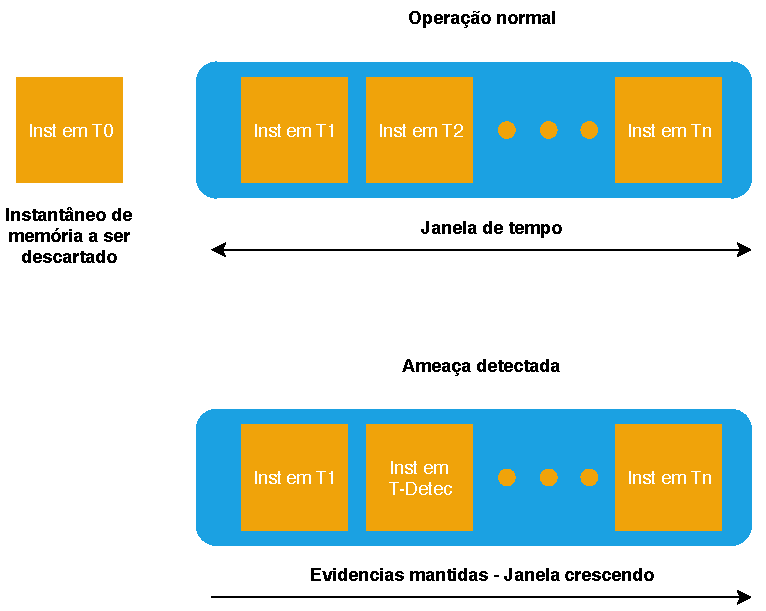
\includegraphics[scale=1.00]{janela.pdf}
\centering
\label{fig:janela}
\begin{center}
Fonte: Próprio autor 
\end{center}
\end{figure}

A maioria das técnicas forenses mais usadas atualmente são voltadas à obtenção da informação em sua totalidade.
%
Isso comumente é feito via cópia bit a bit ou por meio da obtenção do \textit{hardware} físico \cite{SimouCloudChlng:2014} \cite{BemPastPresentFuture:2008}. 
%
Embora tais técnicas possam parecer interessantes à primeira vista, estas muitas vezes acabam sendo responsáveis por um problema: o crescente volume de informações que os investigadores precisam analisar \cite{QuickIncreaseVolumeImpact:2014}.
%
Para mitigar essa dificuldade, em \fancyname são adotadas duas estratégias: a primeira é a definição de um volume de dados que possa ser considerado \textit{suficiente} para a realização de uma investigação; a segunda é a definição de uma \textit{idade máxima} para a evidência enquanto o sistema trabalha em condições normais, isto é, quando não está sob ataque.
%
Para detectar e analisar intrusões na memória de processos, é necessário ter uma cópia da memória antes e depois da intrusão \cite{CaseMemoryForensics:2014}. 
%
Assim, a solução proposta implementa uma janela de instantâneos de memória cobrindo um intervalo de tempo pré-definido, como ilustrado na Figura \ref{fig:janela}. 
%
Em condições normais de operação, as evidências são coletadas com certa periodicidade e coletas que atingem uma determinada idade são descartadas.
%
Em contraste, após a detecção de um evento de ataque (e.g., por um sistema de detecção de intrusões), \fancyname deixa de descartar as coletas mais antigas do \textit{log} de monitoramento.
%
Como resultado, é possível conhecer o sistema antes e depois do ataque e, assim, avaliar sua evolução.
%
%\marcosR{Não sei por que você está utilizando $\backslash\backslash$ no final das suas frases, mas pare de fazer isso... deixe o LaTeX se virar com a formatação. No final, quando você tiver tudo escrito, aí pode fazer algum sentido se preocupar com formatação, mas não antes disso... - Hamilton: é pra formatação mesmo :-) OK vou deixar o latex se virar}
%

\section{Garantindo integridade, confidencialidade e protegendo privacidade e jurisdição}
\label{sec:proposal-desc-chain-of-custody}

%\marcosT{Essa frase não faz sentido: não se ``assina'' nada com um ``hash''. Você pode ``calcular o hash'' ou ``assinar um dado'' (e.g., um dado juntamente com o hash de alguma coisa). Revise essa frase... - Hamilton: Feito}
Finalmente, para persistir a relação evidência-origem e garantir a sua integridade, \fancyname calcula o \textit{hash} $H$ do par \{evidência, identificador da imagem do contêiner\} e armazena a tripla \{$H$, identificador do recurso, evidência\}.
%
Adicionalmente, a presente proposta evita eventuais problemas com o armazenamento desses dados em países com jurisdições diferentes daquelas que devem ser aplicadas na investigação em questão.
%
Especificamente, as evidências coletadas são armazenadas em um local físico fora da nuvem, após serem transportadas por meio de um canal seguro (e.g., via TLS (\textit{Transport Layer Security} -- Camada de Transporte Seguro) \cite{DierksT2008}).
%
%Evitando assim problemas de relacionados a falta de acordos de cooperação no combate a crimes digitais entre regiões onde ocorreu o crime e onde a evidência está armazenada.
Dando ao processo de investigação maior celeridade uma vez que a coleta das evidências já terá ocorrido de forma forensicamente aceitável.
%

\section{Implementação}
\label{sec:proposta-impl}

%\marcosT{CLAREZA: quais ataques? Onde estão esses objetivos (diga a seção!!!)? Perceba que não tem qualquer seção com esse nome: você espera realmente que o leitor procure no seu texto onde eles estão...? - Hamilton: Feito}

\begin{figure}[htb!]
\footnotesize
\caption{Arquitetura geral da solução Dizang}
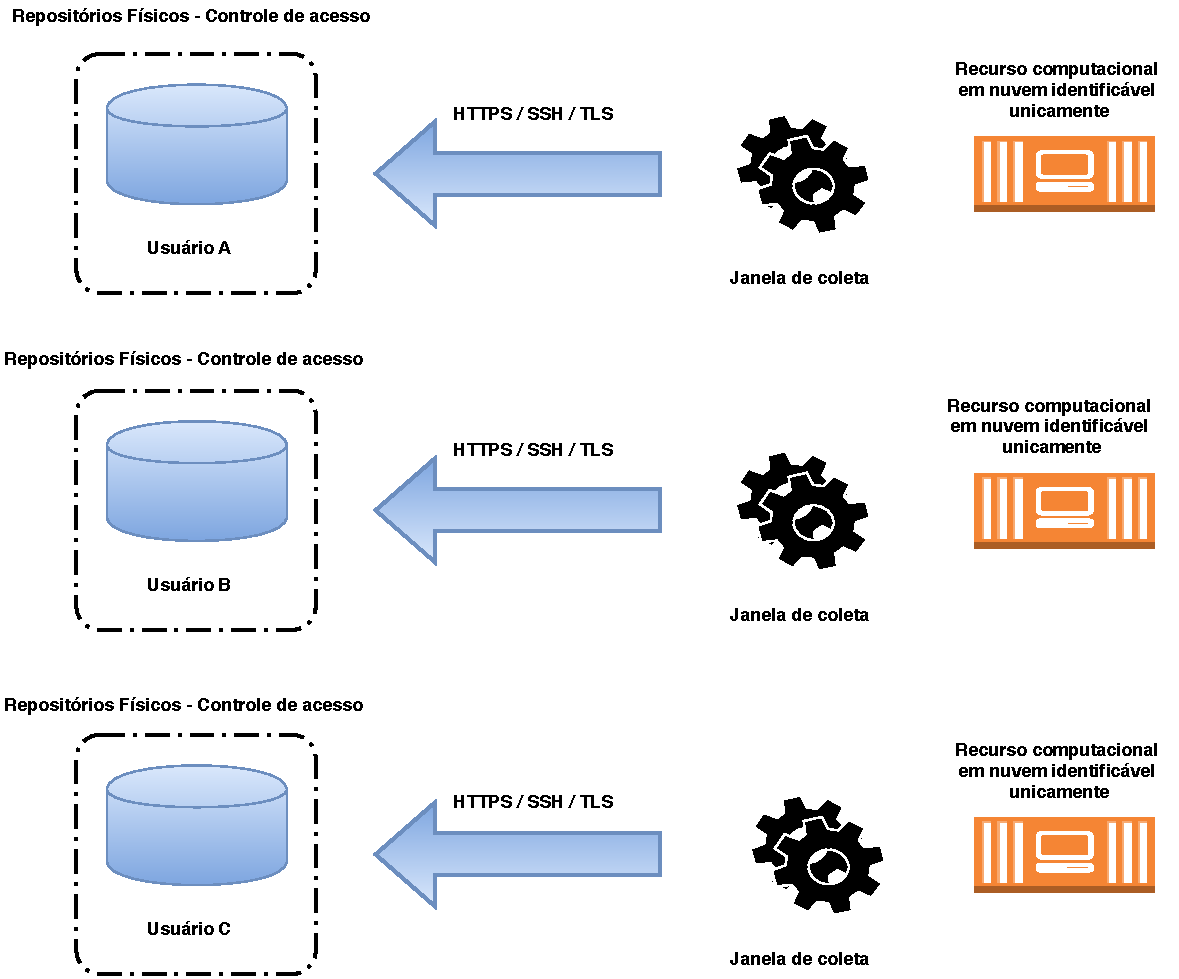
\includegraphics[scale=0.70]{Solucao.pdf}
\centering
\label{fig:Solucao}
\begin{center}
Fonte: Próprio autor 
\end{center}
\end{figure}

%
Os mecanismos propostos foram implementados em uma plataforma de testes visando avaliar a eficácia de \fancyname em coletar as informações de memória dos contêineres de forma reprodutível, sem violar jurisdições ou a privacidade de usuários e a capacidade de detectar injeção de código usando as evidências coletadas.
%
A solução, ilustrada na Figura \ref{fig:Solucao}, consistiu na utilização do serviço EC2 para criação de uma instancia t2.micro Ubuntu Server 14.04 LTS de 64 bits (x86) com armazenamento em SSD na zona Ohio da AWS. 
%na criação de 1 VM usando o Oracle Virtual Box 5.0%\cite{VirtualBox} em um notebook Intel i5 de 2.30Mhz e 4Gb de RAM com sistema operacional de 64 bits.
%
Nesta instância AWS foi manualmente instalado o Docker Engine 1.10 e a API Docker 1.21, com os quais foram criados 3 contêineres executando o Nginx 1.0 em diferentes portas. 
%
Não foram utilizados serviços de contêiner do provedor AWS como EKS ou ECS nos experimentos.
%
Foi desenvolvida uma aplicação Java cujo fluxo é ilustrado na Figura \ref{fig:fluxo-dizang} que, executada no sistema operacional hospedeiro, descobre o identificador de processo associado a cada contêiner, copia o conteúdo do \textit{descritor de alocação de memória não uniforme} (\textbf{/proc/pid/numa\_maps}), o qual contém a alocação das páginas de memória, os nós que estão associados a essas páginas, o que está alocado e suas respectivas políticas de acesso \cite{UnixManPagesNumaMaps}.
%
A cópia e gravação do arquivo é tal que, a cada intervalo de tempo $t$, a aplicação (1) pausa o contêiner em questão, (2) copia a diretório \textbf{numa\_maps}, (3)  concatena os dados obtidos com o identificador da imagem e do contêiner, (4) calcula o $H$ do conjunto e (5) salva o resultado em um arquivo cujo nome é o identificador da imagem e do contêiner e a extensão é \textbf{.mem}. 
%
O transporte seguro da evidência para um armazenamento físico fora da AWS foi implementado usando no serviço EC2, uma instância t2.micro Ubuntu Server 14.04 LTS de 64 bits (x86) com armazenamento em SSD na zona Ohio da AWS no qual foi instalado um servidor \textit{OpenVPN}.
%
Como uma forma básica de controle de acesso, a instância EC2 que contém as evidências foi configurada para aceitar conexões apenas de máquinas nesta VPN.
%
A instância EC2 e a instância da qual foram coletadas as evidências estavam na mesma VPC padrão da AWS
%
Uma máquina física fora da AWS, usou o cliente do \textit{OpenVPN} para estabelecer uma conexão VPN com a instância que contém as evidências e as transportou para o disco da máquina física.
%
A conexão entre a máquina física fora da nuvem e a instância de EC2 na nuvem foi feita utilizando um provedor de banda larga de uso doméstico de 50Gb (Live Tim).
%
Após a conclusão do processo de transporte, a máquina física verifica se existem arquivos \textbf{.mem} em disco mais antigos que um certo intervalo de tempo $t$, descartando-os.
%

\begin{figure}[htb!]
\footnotesize
\caption{Fluxo de execução de Dizang para 1 hospedeiro de contêiner}
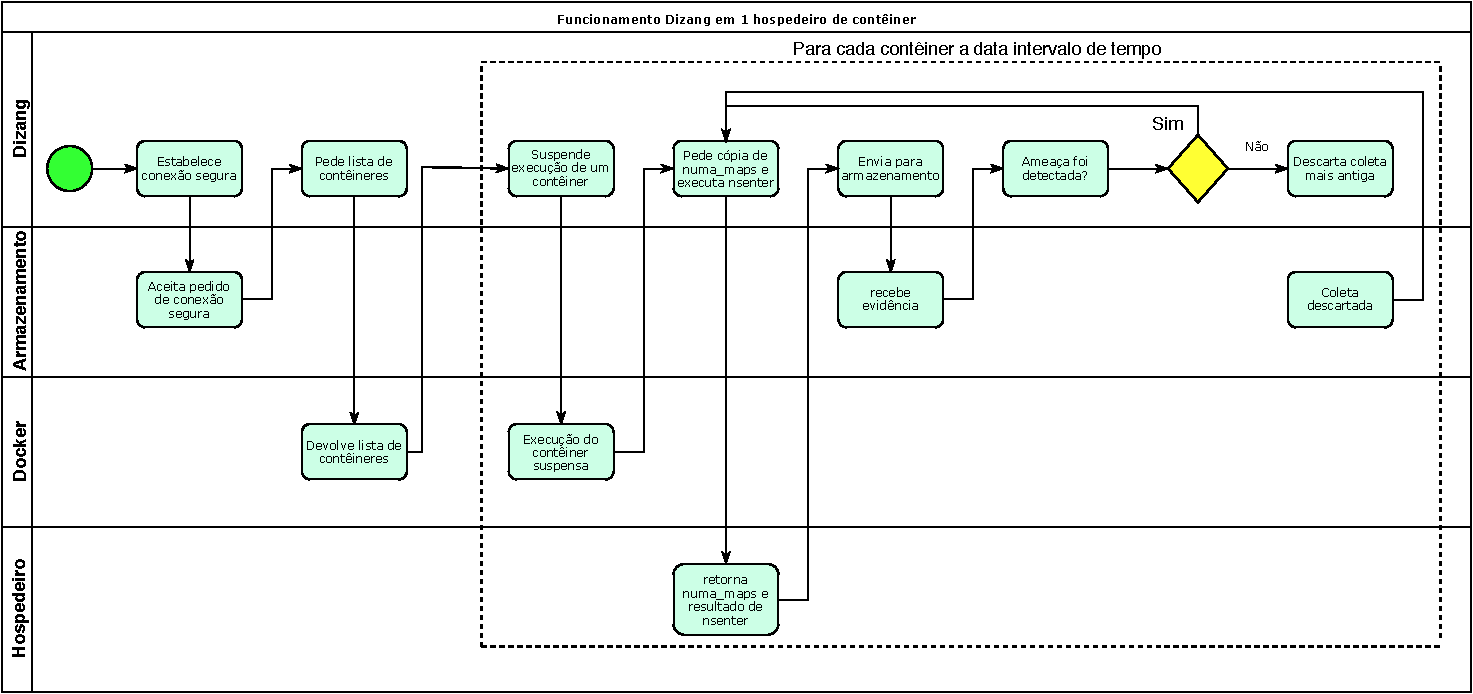
\includegraphics[scale=0.64]{Fluxo-Dizang.pdf}
\centering
\label{fig:fluxo-dizang}
\begin{center}
Fonte: Próprio autor 
\end{center}
\end{figure}


\section{Resultados experimentais}
\label{sec:proposta-exp}

Para avaliar a efetividade de \fancyname na coleta de evidências e identificação de injeção de código, dois experimentos foram realizados usando o ambiente implementado (descrito na Seção \ref{sec:proposta-impl}).
%


\subsection{Análise do desempenho}
\label{sec:proposta-exp-desempenho}

No primeiro experimento, o sistema foi configurado para realizar coletas de memória em intervalos de 1 minuto, salvá-las em armazenamento externo à nuvem e apagar amostras coletadas há mais de 5 minutos. 
%
O sistema foi então executado por 30 minutos, tempo durante o qual foram coletadas como métricas (1) o uso de espaço em disco utilizado pelos instantâneos de memória salvos, (2) o tempo de pausa no contêiner necessário para a cópia delas e (3) o tempo de transporte das evidências para o armazenamento externo a nuvem.


A evolução do espaço em disco ocupado pelos instantâneos de memória, acompanhado através da execução do comando \texttt{du -sh *.mem} do \textit{Unix} no disco de armazenamento externo, é mostrada no gráfico da Figura \ref{fig:evolucao-coleta}.
%
Neste experimento os instantâneos de memória tem 244kb de tamanho. 
%
O gráfico mostra que o aumento do uso do espaço de armazenamento é linear e o crescimento se interrompe quando é atingido o limite de tempo configurado para a janela, pois as coletas com tempo de vida maior que tal limite são apagadas do armazenamento final. 
%
Assim, a solução mantém sob controle o espaço em armazenamento ocupado pelas amostras coletadas.
%
Ao mesmo tempo, instantâneos de memória salvos pela solução depois que os contêineres são removidos continuam no armazenamento da máquina, podendo ser associados a sua origem (i.e., contêiner e imagem), conforme esperado para uma análise forense.
%
Essa capacidade se mantém após a detecção de uma ameaça, pois nesse caso coletas mais antigas deixam de ser apagadas.
%
Logo, é possível descrever o estado do sistema antes e depois do incidente \cite{CaseMemoryForensics:2014}, permitindo-se, por exemplo, que ataques de injeção de código em memória sejam analisados.



%\marcos{EVITE REDUNDÂNCIA ENTRE GRÁFICO E TABELA. Faz sentido apenas se um deles for trazer informações adicionais (e, nesses casos, em geral o gráfico/tabela acaba tendo algum highlight, para deixar a utilidade dessa redundância)
%\begin{table}[htb!]
%\centering
%\caption{Evolução do uso do espaço em disco}
%\label{tab:results-size}
%\begin{tabular}{c|c}
%\hline
%Tamanho total ocupado (KBytes) & Tempo (segundos) \\ \hline
%240                            & 1                \\ \hline
%480                            & 2                \\ \hline
%720                            & 3                \\ \hline
%960                            & 4                \\ \hline
%1200                           & 5                \\ \hline
%1200                           & 6                \\ \hline
%1200                           & 7                \\ \hline
%1200                           & 8                \\ \hline
%1200                           & 9                \\ \hline
%1200                           & 10                \\ \hline
%1200                           & 11                \\ \hline
%1200                           & 12                \\ \hline
%1200                           & 13                \\ \hline
%1200                           & 14                \\ \hline
%1200                           & 15                \\ \hline
%1200                           & 16                \\ \hline
%1200                           & 17                \\ \hline
%1200                           & 18                \\ \hline
%1200                           & 19                \\ \hline
%1200                           & 20                \\ \hline
%1200                           & 21                \\ \hline
%1200                           & 22                \\ \hline
%1200                           & 23                \\ \hline
%1200                           & 24                \\ \hline
%1200                           & 25                \\ \hline
%1200                           & 26                \\ \hline
%1200                           & 27                \\ \hline
%1200                           & 28                \\ \hline
%1200                           & 29                \\ \hline
%1200                           & 30                \\ \hline
%\end{tabular}
%\end{table}

\begin{figure}[htb!]
\footnotesize
\caption{Evolução do uso do espaço em armazenamento com o Dizang}
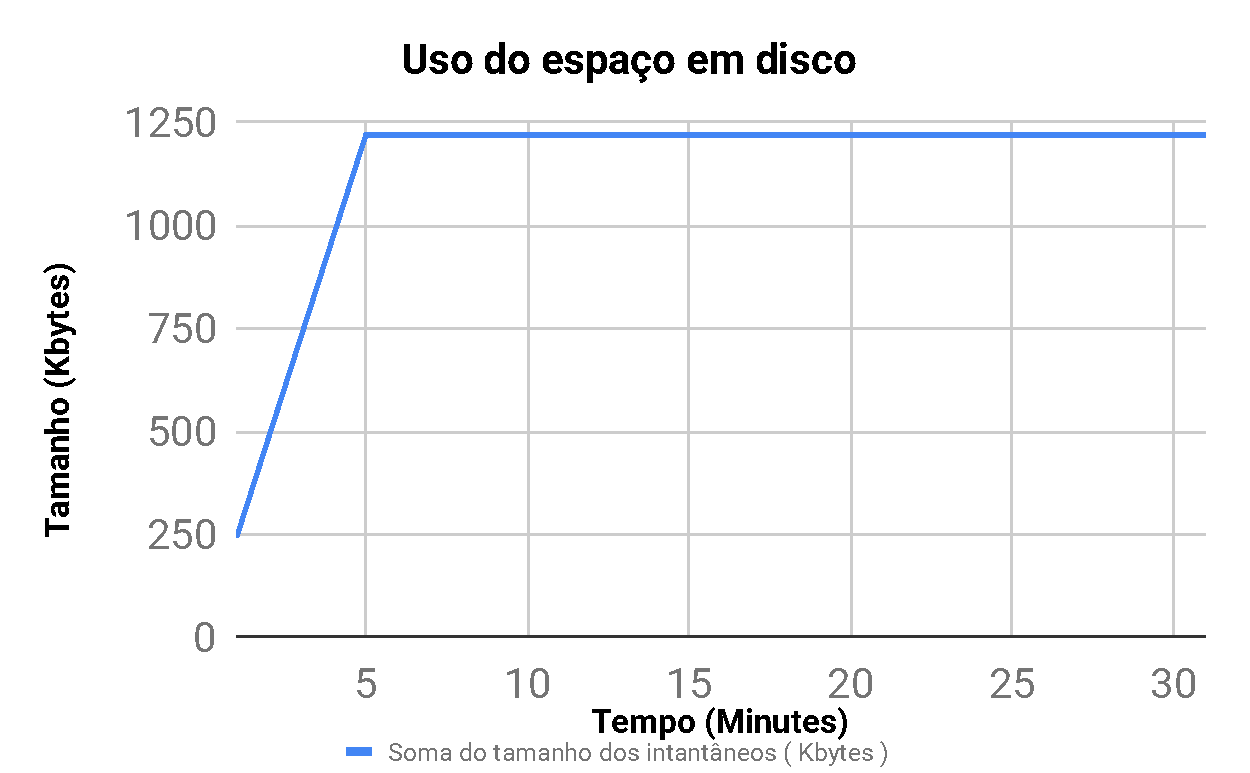
\includegraphics[scale=0.60]{evolucao-coleta.pdf}
\centering
\label{fig:evolucao-coleta}
\begin{center}
Fonte: Próprio autor 
\end{center}
\end{figure}


\begin{comment}
A Figura \ref{fig:memoria_salva}, por sua vez, mostra uma listagem de alguns dos instantâneos de memória salvos pela solução depois que os contêineres são removidos. 
%
Nela pode-se ver que as coletas continuaram no disco da máquina mesmo após a remoção dos contêineres. 
%
Usando o identificador do contêiner e da imagem, consegue-se associar a evidência a sua origem (i.e., a imagem e o contêiner), conforme esperado para uma análise forense.
%
Essa capacidade se mantém após a detecção de uma ameaça, pois nesse caso coletas mais antigas deixam de ser apagadas.
%
Assim, é possível descrever o estado do sistema antes e depois do incidente \cite{Case_Memory_Forensics:2014}, permitindo-se, por exemplo, que ataques de injeção de código em memória sejam analisados.


\begin{figure*}[htb!]
\footnotesize
\caption{Exemplo de lista de instantâneos de memória.}
\fbox{
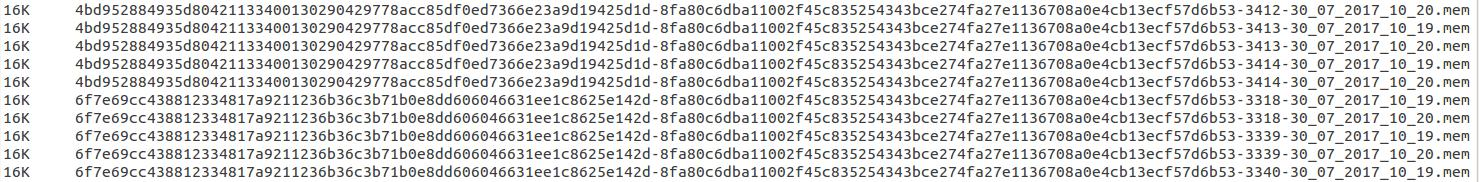
\includegraphics[scale=0.30]{memoria_salva.jpg}
}
\centering
\label{fig:memoria_salva}
\end{figure*}

\end{comment}

%No evento da detecção de uma ameaça a presente proposta deixa de apagar as coletas mais antigas. 
%
%Desta forma é capaz de descrever a história das alterações da memória do contêiner e com isso viabilizar a análise forense em busca das 4 vulnerabilidades de injeção de código em memória citadas no início do artigo. \marcos{Link bem fraco com introdução... pra que explicar em *detalhes* as vulnerabilidades na Introdução se você vai fazer uma explicação *superficial* de como elas são abordadas... Coloquei en passant para não dar a impressão de que você quis chamar a atenção para aquelas vulnerabilidades (sim, eu tinha pedido para você fazer esse link, mas um link tão fraco joga CONTRA você, não a favor...)}
%
%A viabilidade se dá pois consegue descrever o estado do sistema antes e depois do incidente \cite{Case_Memory_Forensics:2014}.
%

Uma potencial limitação da solução proposta é que a pausa de um contêiner para coleta de dados poder, em princípio, causar perdas no desempenho da aplicação sendo executada. 
%
Para avaliar esse impacto, durante o experimento foram medidos os tempos de cópia da memória do contêiner.
%
Os resultados são mostrados no gráfico da Figura \ref{fig:memoria-copia}.
%
É possível notar que, após a inicialização da aplicação, o tempo para realizar a cópia é bastante reduzido, variando entre 20 e 40 milissegundos. 
%
Em especial, para contêineres executando um motor de páginas web dinâmicas, como é o caso do experimento em questão, essa latência deve ser pouco perceptível por usuários finais.
%
Para os casos em que a interrupção da execução do recurso computacional mesmo por breves momentos cause problemas de disponibilidade, é possível realizar o procedimento de coleta em instantes de tempo separados.
%
Assim, ao invés de suspender a execução de todos os recursos computacionais para realização da coleta simultaneamente, o procedimento interrompe-as sequencialmente.
%
Desta forma, a latência demonstrada pode ser considerado o pior caso neste experimento.

\begin{figure}[htb!]
\footnotesize
\caption{Tempo de cópia da memória de um contêiner}
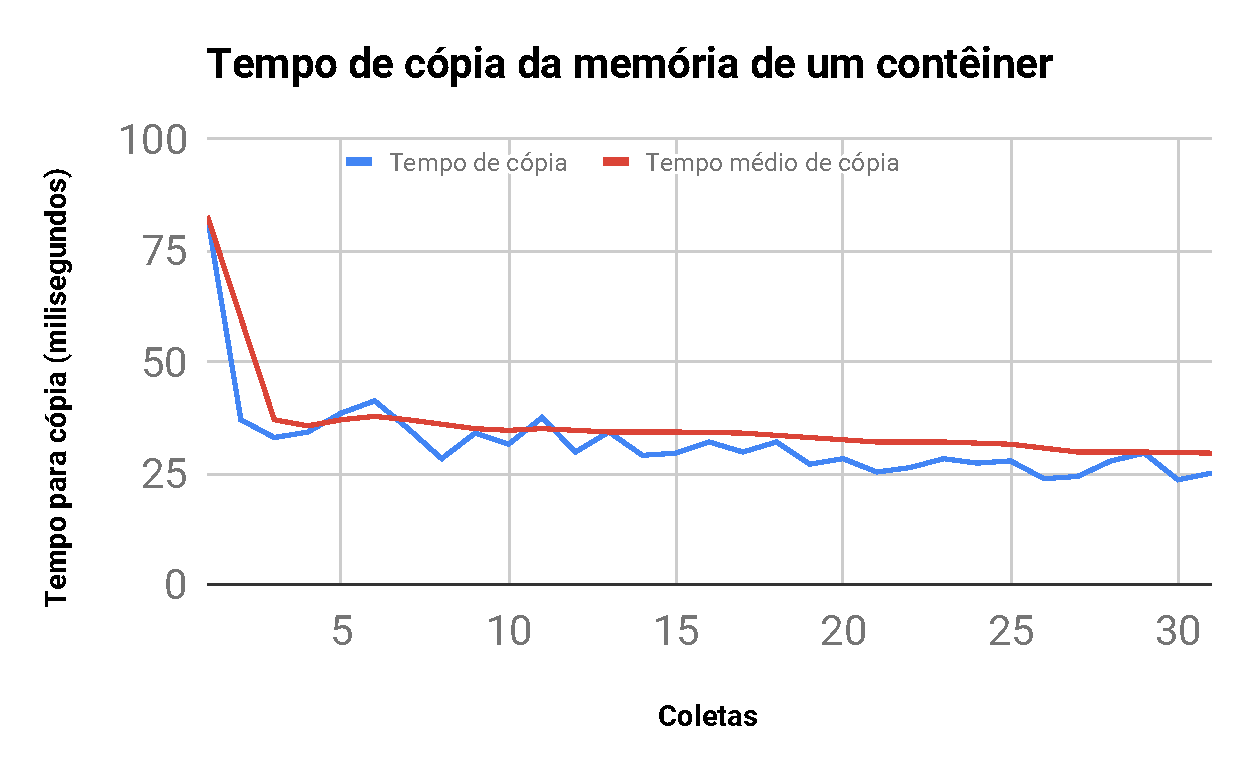
\includegraphics[scale=0.70]{memoria-copia.pdf}
\centering
\label{fig:memoria-copia}
\begin{center}
Fonte: Próprio autor 
\end{center}
\end{figure}


Outra preocupação é o tempo de transporte das evidências para o armazenamento fora da nuvem.
%
Caso o transporte da evidência leve mais tempo que a geração do próximo instantâneo, um \textit{backlog} de transporte se formará levando a perdas nas evidências que estejam pendentes para transporte.
%
Para avaliar esse impacto, durante o experimento foram medidos os tempos de transporte das evidências para o armazenamento fora da nuvem.
%
Os resultados são mostrados no gráfico da Figura \ref{fig:evidencia_transporte}.
%
É possível notar que o tempo de transporte estabiliza após atingido o tamanho da janela. O tempo de transporte da evidência fica, em média próximo dos 30 segundos. 

\begin{figure}[htb!]
\footnotesize
\caption{Tempo de transporte da evidência}
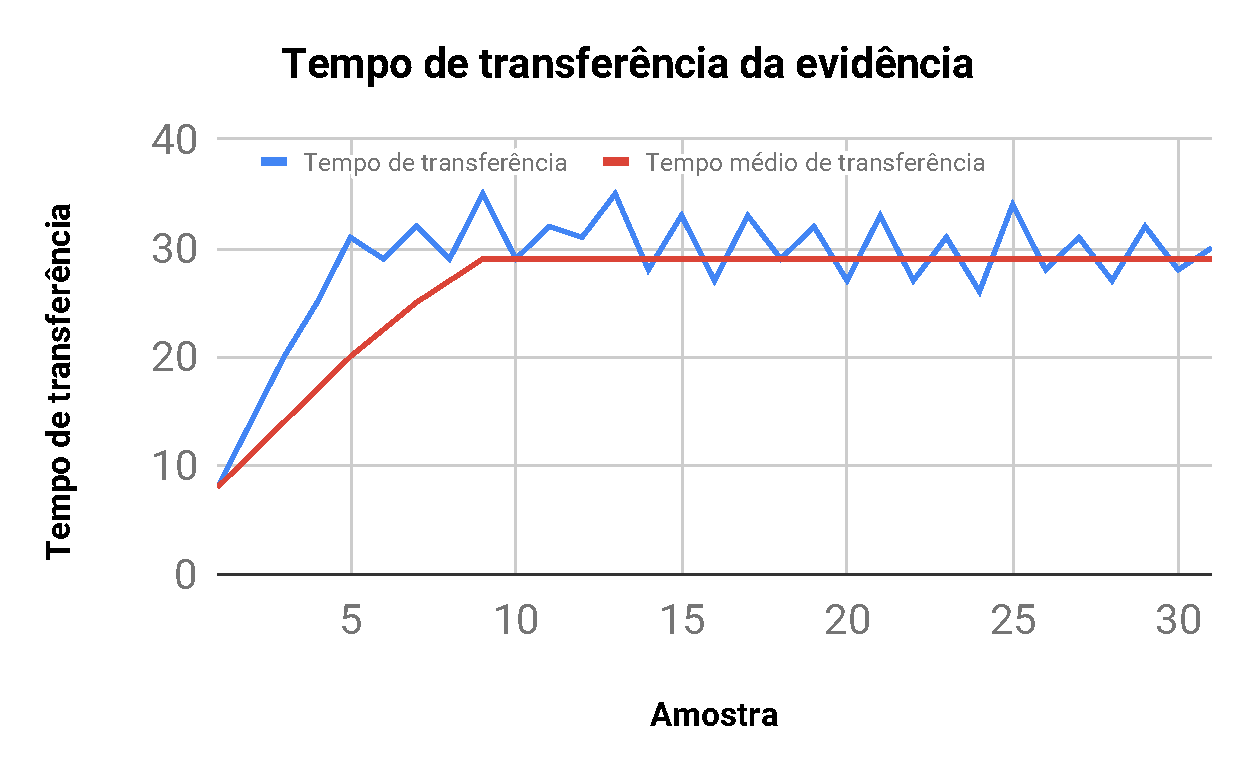
\includegraphics[scale=0.70]{evidencia-download.pdf}
\centering
\label{fig:evidencia_transporte}
\begin{center}
Fonte: Próprio autor 
\end{center}
\end{figure}


%
Tanto a topologia quando a arquitetura do transporte da evidência e a arquitetura do que se deseja extrair a evidência são fatores que contribuem tanto positiva quando negativamente no tempo de transporte.
%
Neste experimento o gerador de evidências, um motor de páginas dinâmicas, está na América do Norte enquanto que a máquina física para onde as evidências foram transportadas e que é responsável pelo transporte da evidência está na América do Sul.


\subsection{Identificação de injeção de código malicioso}
\label{sec:proposta-exp-malware}

Um segundo experimento teve como objetivo determinar se é possível, através da análise das evidências coletadas, identificar injeção de código malicioso na memória do contêiner.
%
Para este fim uma biblioteca \textbf{libexample.so} simulando um código malicioso foi injetado em um dos contêineres.
%
Após cinco minutos de \fancyname realizando coletas, uma biblioteca foi injetada na memória de um dos contêineres. Após a injeção permitiu-se que a solução continuasse coletando por mais 5 minutos.
%
Além da coleta do conteúdo do diretório \textbf{/proc/pid/numa\_maps}, realizou-se também uma cópia crua da memória do processo do contêiner utilizando o utilitário \textit{nsenter} via comando descrito na Figura \ref{fig:comando-copia}.

\begin{figure}[htb!]
\footnotesize
\caption{Comando para cópia crua da memória do processo do contêiner}
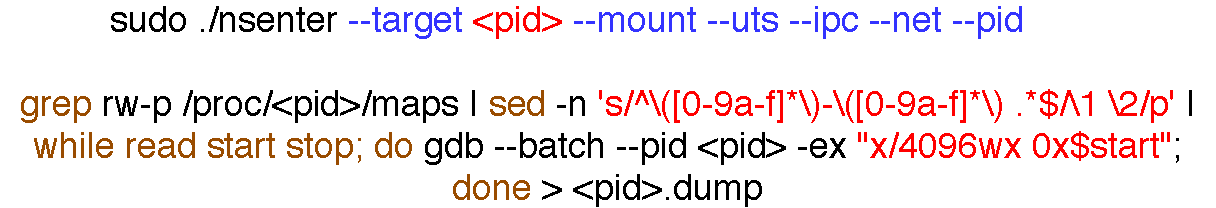
\includegraphics[scale=0.60]{comando-copia-memoria-gdb.pdf}
\centering
\label{fig:comando-copia}
\begin{center}
Fonte: Próprio autor 
\end{center}
\end{figure}

%
De posse das coletas do diretório \textbf{/proc/pid/numa\_maps} comparou-se dois momentos distintos na vida do contêiner, antes e depois da injeção da biblioteca.
%
Observando as Figuras \ref{fig:antes-injecao} e \ref{fig:apos-injecao} é possível notar que no instantâneo após a injeção aparece a biblioteca \textbf{libexample.so} simulando o código malicioso entre os endereços \textbf{7f85631b8000} e \textbf{7f85633b9000}.
%
Logo, é possível identificar a injeção de um código malicioso via evidência coletada por \fancyname do diretório \textbf{/proc/pid/numa\_maps}, permitindo-se por exemplo que ataques de injeção de código sejam identificados.
%
A Figura \ref{fig:conteudo-memoria-copia-gdb} mostra o conteúdo da parte legível da memória no endereço \textbf{0x7f85633b9000} onde a biblioteca \textbf{libexample.so} simulando um código malicioso está alocada.

\begin{figure}[htb!]
\footnotesize
\caption{Parte do arquivo \textbf{/proc/pid/numa\_maps} ANTES da injeção }
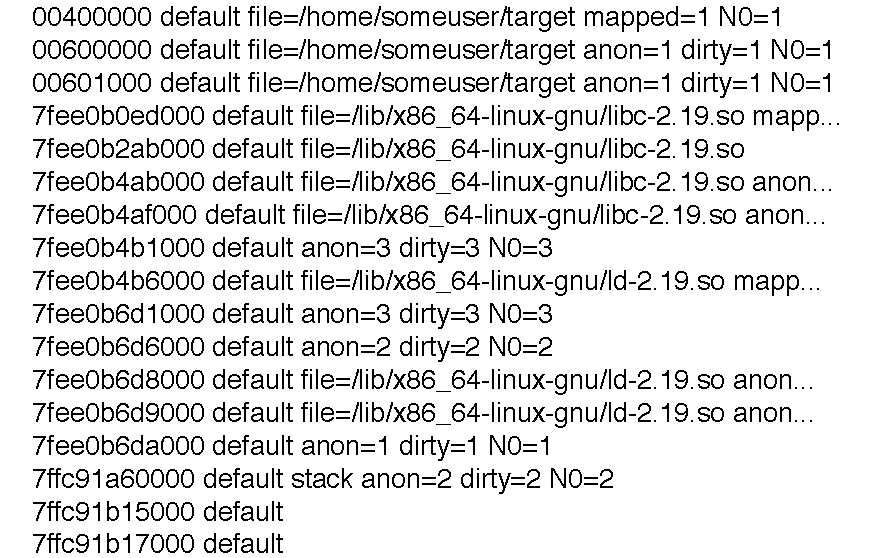
\includegraphics[scale=0.80]{antes-injecao.pdf}
\centering
\label{fig:antes-injecao}
\begin{center}
Fonte: Próprio autor 
\end{center}
\end{figure}


\begin{figure}[htb!]
\footnotesize
\caption{Parte do arquivo \textbf{/proc/pid/numa\_maps} APÓS a injeção }
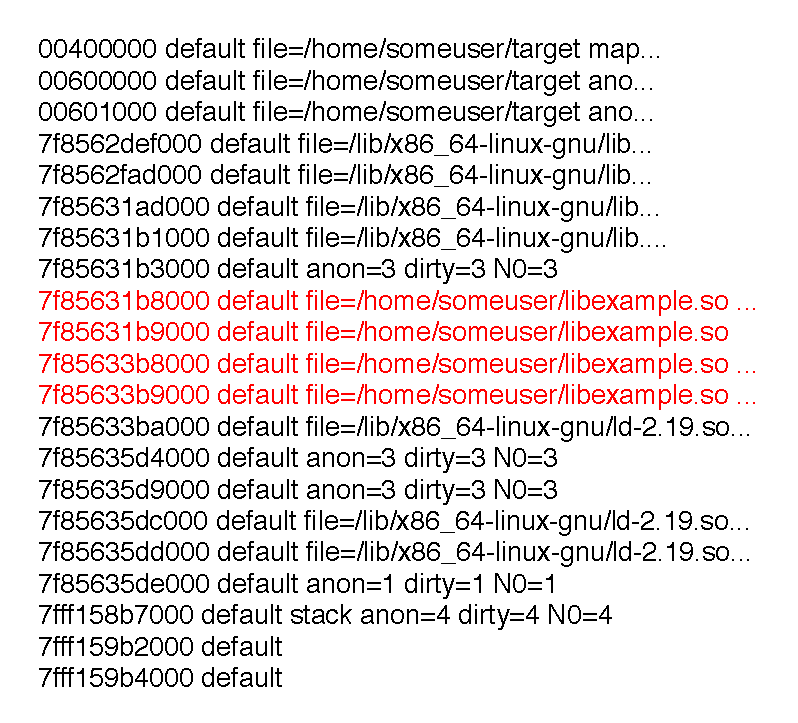
\includegraphics[scale=0.80]{apos-injecao.pdf}
\centering
\label{fig:apos-injecao}
\begin{center}
Fonte: Próprio autor 
\end{center}
\end{figure}

%
%As primeiras tentativas de cópia do conteúdo da memória do processo do contêiner foram feitas via \textit{ptrace} e não obteve sucesso. 
%
%Segundo \cite{cgroupsxptrace} isto ocorre pois as chamadas de sistema que ferramentas como \textit{ptrace} e \textit{htop} usam foram criadas antes da implementação de \textit{cgroups} no \textit{kernel} do linux e sendo assim não tem consciência da existência de isolamento entre processos.
%
%Quando o \textit{ptrace} tenta acessar uma área de memória isolada por \textit{cgroups}, o \textit{kernel} envia um sinal de violação de acesso de memória, o resultado é mostrado na Figura \ref{fig:erro-copia-gdb}.
%

%A documentação do Docker \cite{capabilities} menciona o comando \texttt{--cap-add=SYS_PTRACE --security-opt-seccomp=unconfined} que permite que o \textit{ptrace} consiga acessar a memória de um processo dentro do contêiner mas não permite que a máquina hospedeira ou outro contêiner tenha acesso (referência).
%
%Ainda segundo \cite{cgroupsxptrace} uma alternativa para viabilizar a monitoração e acesso a informações de memória seria o de expor tais informações na estrutura de \textbf{/sys/fs/cgroup/} da mesma forma que é feita para \textbf{/proc/pid/}.
%
%O sucesso na cópia do conteúdo da memória do processo do contêiner só foi alcançado quando utilizou-se a ferramenta \textit{nsenter}.
%

\begin{figure}[htb!]
\footnotesize
\caption{Conteúdo da memória de \textbf{libexample.so} no formato [endereço]: [conteúdo]}
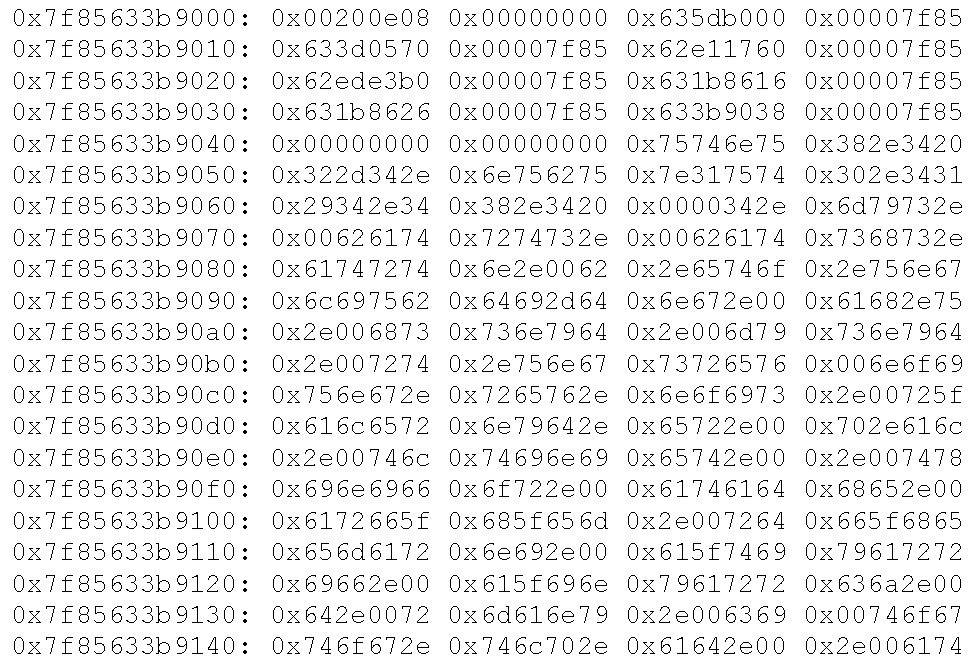
\includegraphics[scale=0.65]{conteudo-memoria-copia-gdb.pdf}
\centering
\label{fig:conteudo-memoria-copia-gdb}
\begin{center}
Fonte: Próprio autor 
\end{center}
\end{figure}


%\begin{figure}[htb!]
%\footnotesize
%\caption{Tentativa mal sucedida de cópia do conteúdo da memória}
%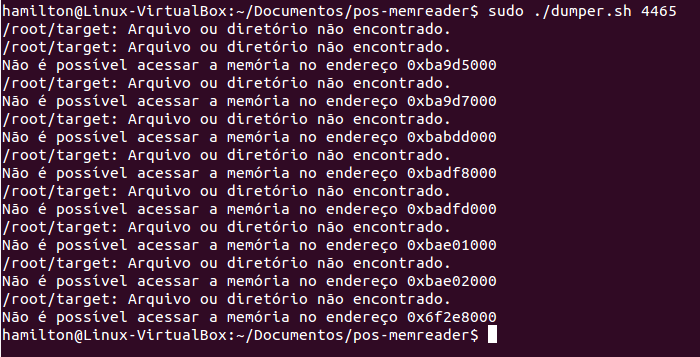
\includegraphics[scale=0.65]{nao-consido-dumpar-memoria.png}
%\centering
%\label{fig:erro-copia-gdb}
%\begin{center}
%Fonte: Próprio autor 
%\end{center}
%\end{figure}


\section{Limitações}
\label{sec:proposta-limit}

A proposta descrita pede que o recurso em nuvem seja identificável de forma única a fim de realizar a associação entre evidência e sua origem.
%
Durante o curso deste projeto essa identificação única só foi possível através do hash da imagem do contêiner. Este foi o único recurso que, submetido ao processo de construção a partir da mesma receita resultou no mesmo \textit{hash} da imagem.
%
Assim, a implementação para verificação da solução proposta consegue apenas coletar informações de memória no espaço do usuário (\textit{user space}), ela não consegue acessar o espaço de núcleo do sistema operacional (\textit{kernel space}). 
%
A implementação de \fancyname neste documento em princípio não consegue investigar códigos malicioso que se baseiam em informações do \textit{kernel space}.
%
Isso inclui, por exemplo, a comparação de informações do PEB (\textit{Process Environment Block} -- Bloco para o Ambiente dos Processos), que ficam no \textit{user space}, com informações do VAD (\textit{Virtual Address Descriptor} -- Descritor de Endereços de Memória Virtual), que fica no \textit{kernel space}. 
%
%Análise de ameaças do tipo DKOM ( \textit{Direct Kernel Object Manipulation} -- Manipulação Direta dos Objetos do Kernel ) também não se beneficiam com a solução aqui proposta. 
%\marcosT{Não entendi a ``associação com o contêiner'' aqui. Você quer dizer que ``não se beneficiam com a solução aqui proposta'' ou outra coisa? Você não definiu o que seria a tal ``associação com o contêiner'' fora do contexto da sua solução, então ficou confuso - Hamilton: Feito}.

Como mencionado em \cite{CaseMemoryForensics:2014}, ``para uma análise eficiente de um incidente em memória, são necessárias cópias da mesma \textbf{antes e depois} do incidente.''
%
Outra limitação da solução proposta é a necessidade da mesma estar instalada no sistema sob investigação a priori para que os resultados descritos neste documento sejam alcançados. 


\chapter{Conclusões e recomendações para trabalhos futuros}
\label{sec:proposta-concl-recom}

%
Neste capítulo são apresentadas as conclusões do presente trabalho e as recomendações para a continuidade dos trabalhos neste campo de estudo.

\section{Conclusões}
\label{sec:proposta-concl}

%\marcosT{Uma boa conclusão retoma, logo na primeira frase, o problema que ela se propunha a resolver. Comece com uma ou mais frases nesse sentido, (nota: \textbf{sem} copiar+colar de outro ponto do texto). - Hamilton: Feito} \marcosT{Só que não: eu disse para você retomar o \textbf{problema} na sua primeira frase. Sua frase começa retomando a \textbf{solução}. Essa que você colocou como primeira seria boa como uma segunda frase, em que você reforça como resolve o problema - Hamilton: Acho que agora foi :)}
%
Ameaças digitais que atuam diretamente na memória de sistema não costumam deixar rastros em disco após terem os recursos correspondentes desalocados, dificultando análises forenses posteriores.
%
Esse problema é especialmente notável em sistemas de computação em nuvem, nos quais a alocação e desalocação de recursos virtualizados (e.g., VMs e contêineres) é frequente.
%
Essa característica, aliada a aspectos como multi-inquilinato e multi-jurisdição de nuvens computacionais, dificulta a coleta de evidências para a investigação de incidentes.

%
Nesse cenário, a proposta apresentada visa relacionar o instantâneo de memória a sua origem, utilizando o \textit{hash} calculado do recurso computacional em nuvem como identificador da origem da evidência armazenada.
%
Para evitar uso excessivo de memória, a quantidade de dados armazenados usa uma janela de armazenamento, o que permite descrever a memória antes e depois de um ataque (e.g., de injeção de memória). 
%
Transportando de forma segura e armazenando a evidência em local conhecido fora da nuvem, evitam-se os problemas relacionados a multi-jurisdição e multi-inquilinato das nuvens computacionais.
%
A comparação de instantâneos de memória coletados em diferentes instantes de tempo permite a identificação de injeção de código assim como extrair o conteúdo da parte legível do endereço de memória correspondente.

%
Combinada com uma ferramenta para identificação de ameaças, essas características de \fancyname o transformam em uma solução poderosa para prover evidências e, assim, viabilizar análises forenses na nuvem.

\section{Trabalhos Futuros}
\label{sec: proposta-trab-fut}

%
Como mencionado em \ref{sec:proposta-limit} a solução proposta é capaz de gerar evidências de memória apenas do espaço do usuário (\textit{user space}). 
%
Alguns códigos malicioso injetados em memória são capazes de manipular o retorno de funções do kernel. Recomenda-se para trabalhos futuros a incorporação à \fancyname uma forma de realizar a extração do conteúdo de memória do espaço do kernel (\textit{kernel space}).